\documentclass[a4paper,english,12pt,bibliography=totoc]{scrreprt}

\usepackage[T1]{fontenc} %immer
\usepackage[utf8]{inputenc} %am
\usepackage{babel} %Anfang

\usepackage{enumitem} %Aufzählungen verändern
\usepackage{comment}
%Gleichungen verwenden
\usepackage{newtxtext}
\usepackage{amsmath}
\usepackage{amssymb}
\usepackage{mathptmx}
%\usepackage{txfonts}

\usepackage{listings}% code blocks
\usepackage[most]{tcolorbox}

%Querverweise
\usepackage{varioref} %immer
\usepackage{hyperref} %in dieser
\usepackage{cleveref} %Reihenfolge

\usepackage{booktabs} %schönere Tabellen
\usepackage{siunitx} %SI-Einheiten
\usepackage{tabularx} %Tabellen mit flexiblen Spalten	

\usepackage{graphicx} %Grafiken verwenden

\usepackage[backend=biber,style=numeric]{biblatex}
\addbibresource{main.bib} 

\usepackage{lipsum} %Blindtext
\usepackage{subcaption}
\usepackage{afterpage}
\usepackage[headsepline]{scrlayer-scrpage} %Paket für Kopfzeilen
\usepackage{afterpage}
\usepackage{float}
\automark[subsection]{section}

\pagestyle{scrheadings}
\ihead{} % oben links
\chead{\leftmark} % oben Mitte
\ohead{} % oben rechts
\cfoot{\pagemark} % unten Mitte
\automark[section]{section} % Modified line

% Zu volle hboxen korrigieren
\tolerance 1414
\hbadness 1414
\emergencystretch 1.5em
\hfuzz 0.3pt
\widowpenalty=10000
\vfuzz \hfuzz
\raggedbottom

%Informationen über das Dokument
%\date{\today}


\begin{document}


\begin{titlepage}
	\centering
	
\includegraphics[width=0.8\textwidth]{logo_uulm_sw}
	
	\vspace{1cm}
	\LARGE Laboratory Module for Master Programs
	\Huge \textbf{Biophysics Lab Course}
	
	\vspace{1cm}
	\Large Experiment:

	\Huge \textbf{Ion channels}
	
	\vspace{15mm}
	\Large Performed on 24.06.2024
	
	\vspace{5mm}
	\LARGE Group 8
	
	\vspace{1cm}
	\Large
	\begin{tabular}{rcl}
	\textbf{Haiyang Zhang} & and & \textbf{Nicolae Turcan}\\
	\href{mailto:student.1@uni-ulm.de}{haiyang.zhang@uni-ulm.de} & & \href{mailto:student.2@uni-ulm.de}{nicolae.turcan@uni-ulm.de}
	\end{tabular}
	
	\vspace{7mm}
	Supervisor: Carlheinz Röcker
	
	\vfill
	\begin{tabular}{p{50mm}@{\hspace{5cm}}p{50mm}}
	\hrulefill & \hrulefill \\
	%\centering Haiyang Zhang  & \centering Nicolae Turcan
	\end{tabular}
	
	\vspace{5mm}
	\normalsize \raggedright
	We hereby confirm that we have elaborated the present work independently and have detailed knowledge of the entire contents.
\end{titlepage}



\tableofcontents

\chapter{Introduction}
\label{cha:Introduction}
\section{Gramicidin A}
%A breif introduction to Gramicidin A, point out that it's structure makes it possible to anchor in the membrane, and two of them works together as an ion channel.
Gramicidin A is a linear peptid consisting of 15 alternating L- and D- amino acids with hydrophobic side chains. Its left hand $\beta$ helix formation projects all hydrophobic side chains outwards, making it a high affinity inside the lipid membrane. Meanwhile, a hydrophilic channel is formed in the centre by the carbonyl groups of the peptide backbone. In a linear dimer, two gramicidin molecules could form a hydrophilic transmembrane pore and enables the cations to travel through.
\begin{figure}[H]
\centering
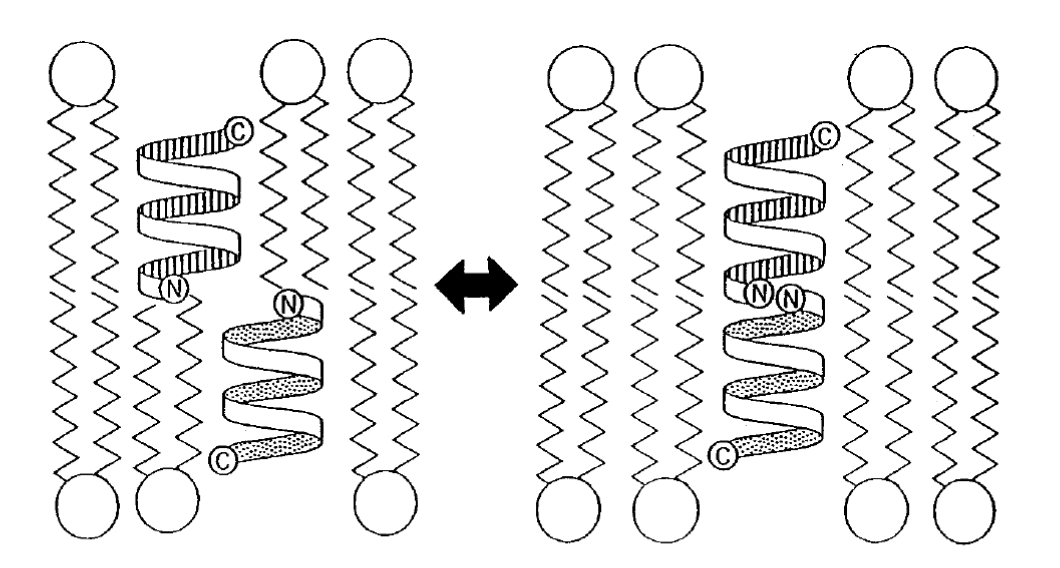
\includegraphics[width = 0.8\textwidth]{Group 8/gramidicin dimer}
\caption{The sketch of the gramidicn monomer and dimer in the membrane}
\end{figure}

\section{Ion transport}
%Introduce what will happen with a single and with multi channels in the membrane and the values could acquire from each gating curve 
Pure lipid membrane seldom permeable for ions. In cells, the ions are transported via the transmembrane channels. For gramicidin channels, the negatively polarized carbonyl groups form an binding sites array for the cations. An kinetic model could be derived by assuming there are only two symmetry binding sites in the channel:
\begin{figure}[H]
\centering
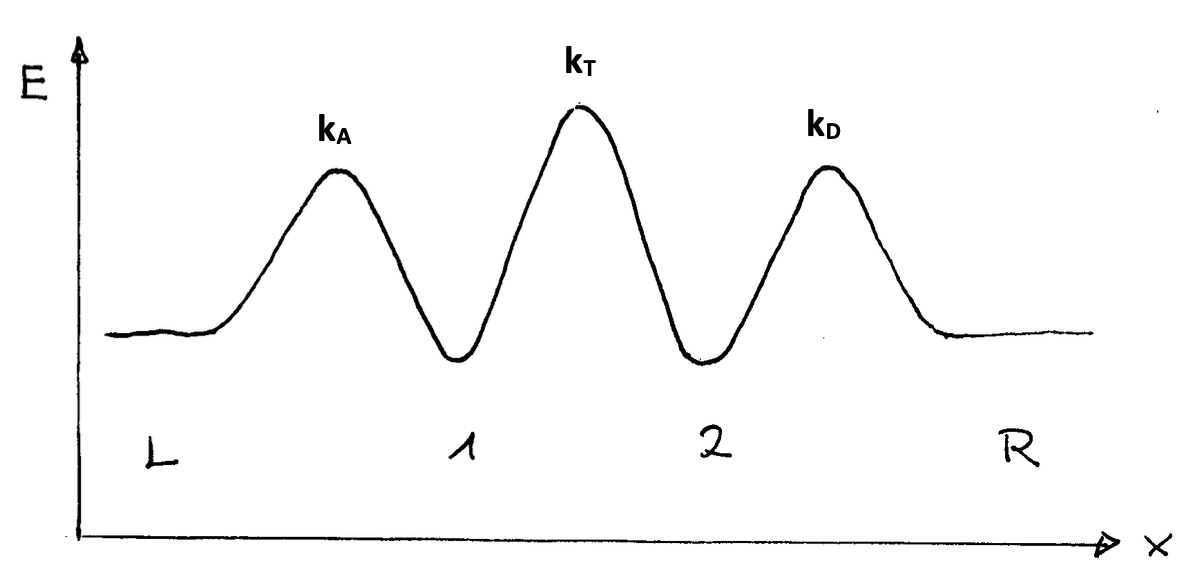
\includegraphics[width = 0.8\textwidth]{Group 8/potential barrier.png}
\caption{Potential plot of the two site binding model}
\end{figure}
Here the k$_A$, k$_T$ and k$_D$ are the rates of binding, transport and dissociation process of the ions, and the barrier height E$^*$ determined the possibility of the ion hopping to another state, where:
\begin{equation}
k = k_0 \cdot e^{-\frac{E^*}{k_bT}}
\end{equation}
If a voltage V$_M$ was applied on the membrane, the energy barrier now is E$^*$ =  V$_M$q. And when the voltage is small, we could acquire the following formulas describe the current through a single ion pore:
\begin{equation}
i_0 = \frac{k_A\cdot c}{2+\frac{k_D}{k_T}}\cdot \frac{q^2}{k_BT}\cdot V_M
\end {equation}
This represents Ohm's law with the single channel conductance:
\begin{equation}
\Lambda = \frac{k_A\cdot c}{2+\frac{k_D}{k_T}}\cdot \frac{q^2}{k_BT}
\end{equation}
which depends on the linear relationship of the ion concentration to the channel numbers N$_p(t)$:
\begin{equation}
I_M(t) = N_p(t)\cdot \Lambda \cdot V_M
\end{equation}
The current steps could be observed if there are one or a few of channels open together. With the chemical dynamic model of the dimerization:
\begin{equation}
 G_1+G_1 \overset{k_A}{\underset{K_D}{\leftrightarrow}} G_2
\end{equation}
We could analyse the dissociation rate of gramidicin dimer channel with the single channel open and close signal, since it should follow the possion interval distribution. For multi channels opening signal, the changing rate is related to both association and dissociation rate, thus we could not calculate the dissociation rate. However, we could still observe the stepwise current distribution.

\section{Autocorrelation analysis}
%For many channel situation, we need an autocorrelation analysis. What is the basic idea of it? And what could we acquire from that?
When there are many channels open and close in short time period, it is impossible to analyze the curve by distinguish the explicit gating values. In this case, we need autocorrelation analysis. The basic idea of autocorrelation analysis is by comparing the similarity of the curve at time t and (t+T) to acquire the properties of the target. In our experiment, we dealt with the current fluctuation around the average current:
\begin{equation}
    x(t) = I(t) - <I>
\end{equation}
Thus, we had the following correlation function:
\begin{equation}
    C(T) = <x(t)\cdot x(t+T)> = <x^2> \cdot e^{-T/\tau} = <(I(t)- <I>)^2> e^{-T/\tau}
\end{equation}
If the gramicidin concentration is relatively low, the relaxation time $\tau$
should equal to the 1/k$_d$, where k$_d$ is the dissociation rate of the gramicidin dimer. In this way, even we could not identify the individual channel in the signals, we can also acquire the dissociation rate. 
\section{Black lipid membrane}
%Briefly describe the theory of it, and maybe also how to make it.
In order to embed the gramicidin ion channels, we used the 'M\"uller-Rudin' method to construct an artificial membrane. The lipid( mono-olein) is dissolved in the long chain hydrocarbon solvent(tetra-decane) at a concentration of 3,5 mg/ml . In the practice, a drop of lipid oil is attached to the opening of a coated hydrophobic glass capillary. The oil would slowly immerse along the hydrophobic glass capillary, leaves the membrane at the entrance becoming thinner. At the beginning, a newton ring could be observed due to the interference of the light reflected from the front and back surface of the membrane. When the membrane is much thinner than the wavelength, Interference of all visible wavelengths will be destructive, and the lipid will be black. Thus the membrane is called black lipid.
\begin{figure}[H]
    \centering
    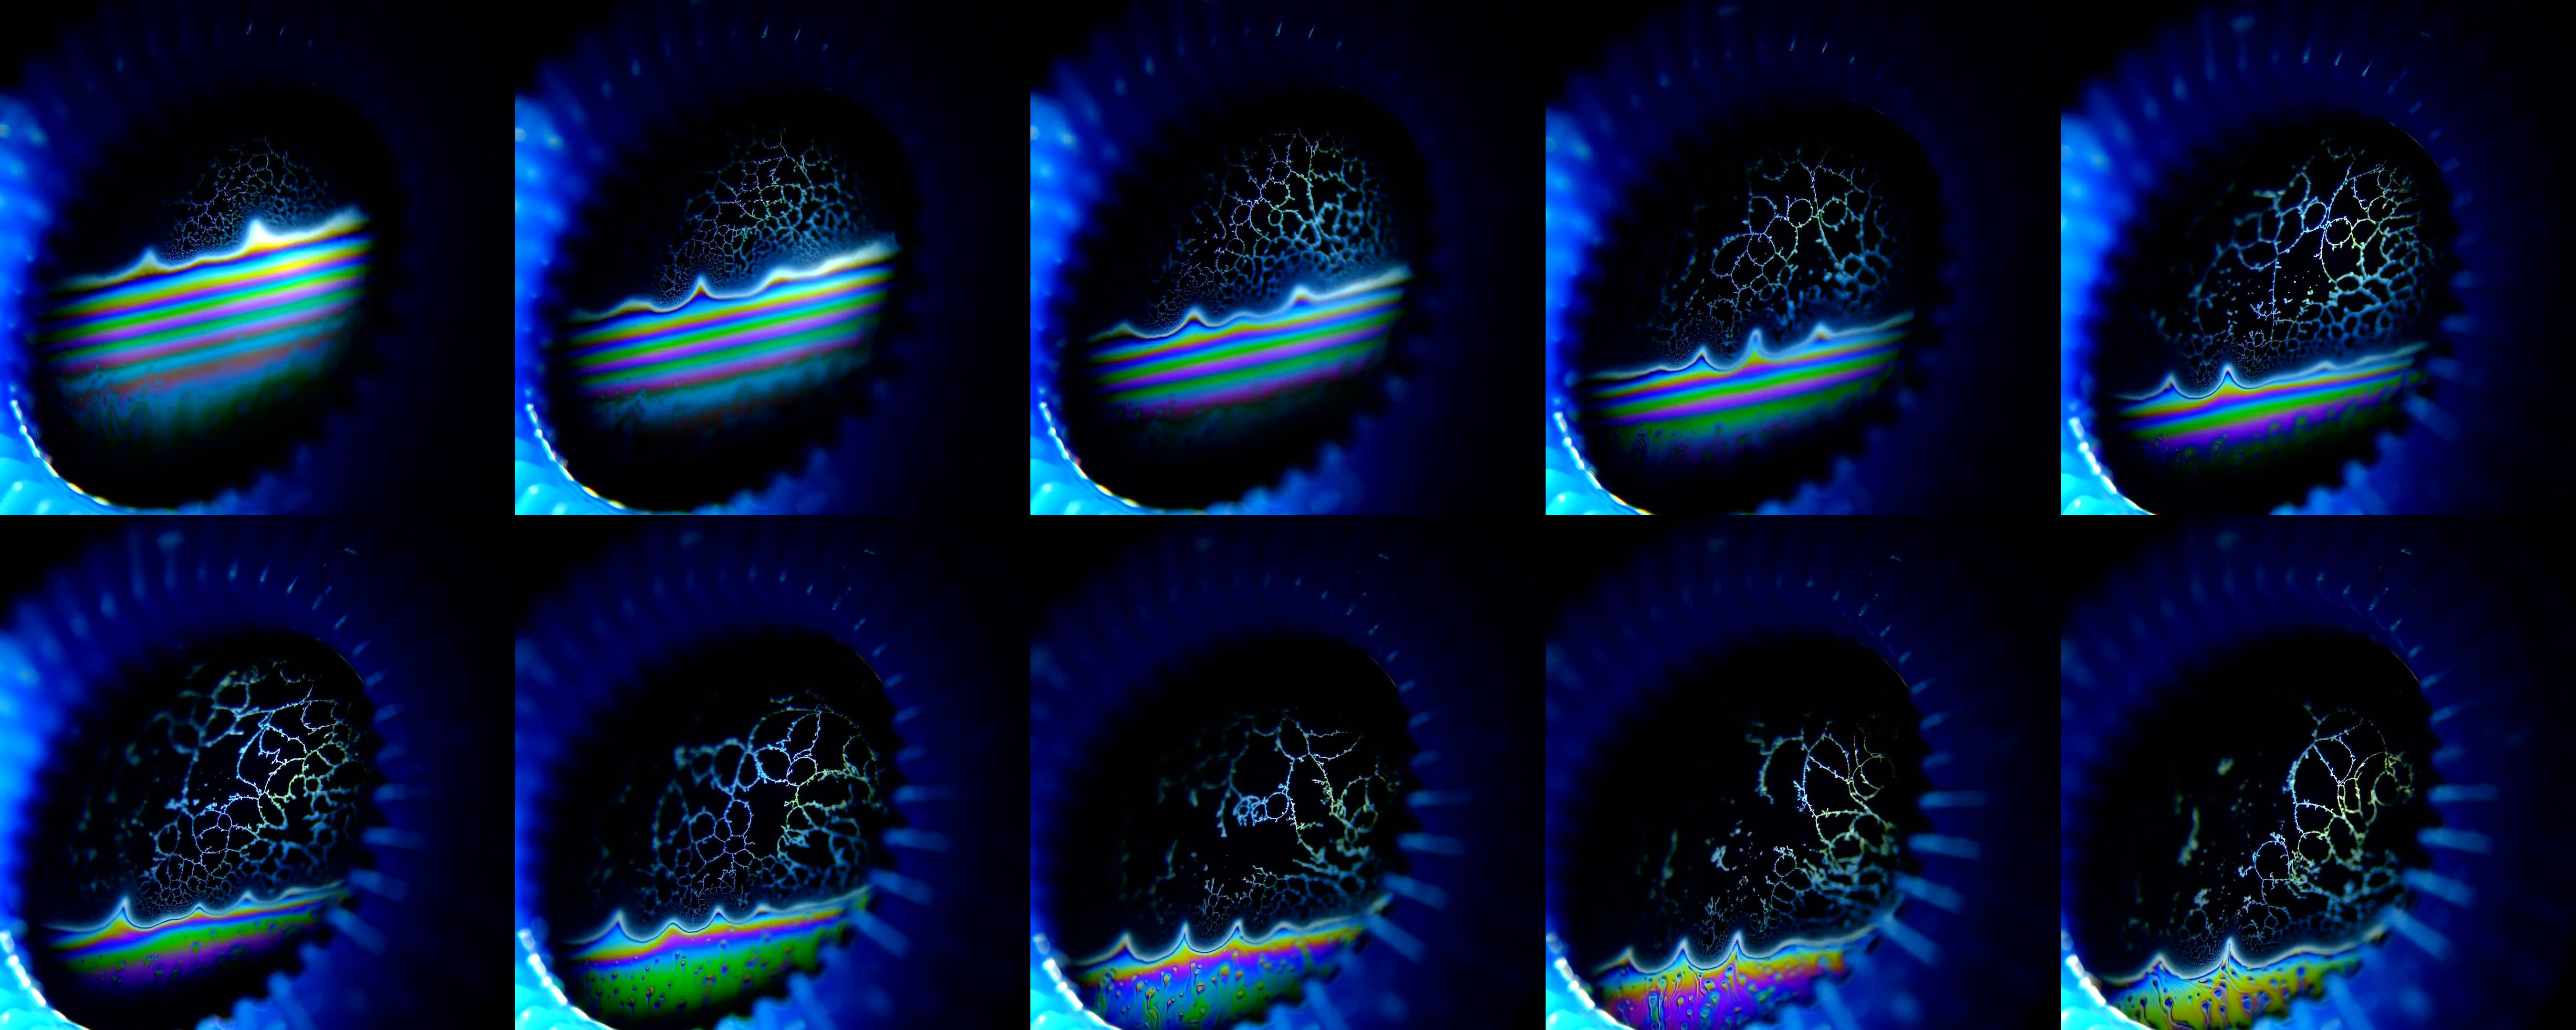
\includegraphics[width = 0.9\textwidth]{Group 8/Black Bubble Membrane.jpg}
    \caption{Timeseries of the membrane thinning process of a soap bubble membrane, photographed by Nicolae Turcan. t = 20s}
    \label{fig:enter-label}
\end{figure}

\begin{comment}
\section{Introduction}
Ion channels are critical components in biological membranes, facilitating the selective transport of ions across the lipid bilayer. These channels are essential for various physiological processes, including the maintenance of cell potential, signal transduction, and ion homeostasis. Gramicidin A is a linear peptide consisting of 15 alternating L- and D-amino acids with hydrophobic (Ala, Leu, Val) or amphiphatic (Trp) side chains&#8203;:citation[oaicite:7]{index=7}&#8203;. In lipid membranes, this peptide forms a left-handed $\beta$-helix, where the hydrophobic side chains project outward, creating a hydrophilic channel in the center by the carbonyl groups of the peptide backbone.

When two gramicidin molecules associate, they form a dimer that spans the hydrophobic core of the lipid membrane, establishing a pore through which ions can pass (Fig.~\ref{fig:gramicidin_pore})&#8203;:citation[oaicite:6]{index=6}&#8203;. The gramicidin dimer has a total length of approximately 2.6 nm and forms a hydrophilic pore about 0.4 nm in diameter&#8203;:citation[oaicite:5]{index=5}&#8203;.

\begin{figure}[h]
    \centering
    \includegraphics[width=0.5\textwidth]{gramicidin_pore.png}
    \caption{Sketch of gramicidin forming a pore in a lipid bilayer by the association of two monomers (adapted from B.A. Wallace, Bioassays 22 (2000) 227)&#8203;:citation[oaicite:4]{index=4}&#8203;.}
    \label{fig:gramicidin_pore}
\end{figure}

The dynamics of ion channel formation and dissociation are stochastic, resulting in channels that fluctuate between open and closed states. This process, known as 'spontaneous gating', can be described by the reaction:

\begin{equation}
G_1 + G_1 \xrightleftharpoons[k_d]{k_a} G_2,
\end{equation}

where $G_1$ represents monomers and $G_2$ represents dimers. The rate constant $k_d$ is the probability per time unit for the dissociation of gramicidin dimers&#8203;:citation[oaicite:3]{index=3}&#8203;.

When few gramicidin molecules are present, the membrane will have either no channel or a single open channel. In such cases, the current through the membrane, at a constant membrane voltage $V_M$, changes in discrete steps corresponding to the formation or destruction of a single channel (Fig.~\ref{fig:current_trace})&#8203;:citation[oaicite:2]{index=2}&#8203;.

\begin{figure}[h]
    \centering
    \includegraphics[width=0.5\textwidth]{current_trace.png}
    \caption{Schematic current trace showing the opening and closing of ion channels due to the dimerization reaction of gramicidin&#8203;:citation[oaicite:1]{index=1}&#8203;.}
    \label{fig:current_trace}
\end{figure}

At higher gramicidin concentrations, individual opening and closing events are not discernible. Instead, the membrane current exhibits noise due to the stochastic nature of these events. The autocorrelation function of this noise can be analyzed to determine channel properties such as the single-channel conductance and the average channel lifetime&#8203;:citation[oaicite:0]{index=0}&#8203;.

In this experiment, we aim to characterize the properties of ion channels formed by gramicidin in a lipid membrane. We will determine the single-channel current and analyze the distribution of channel lifetimes at different membrane voltages. This analysis will allow us to verify Ohm's law for single-channel currents and understand the effects of varying gramicidin concentrations on membrane conductivity.
\end{comment}





\chapter{Experimental Results  and Problems}
\label{cha:Experiment}
\section{Problems}

\subsection{Preparation and characterisation of a lipid membrane}

The preparation of the lipid membrane is described in the introductory part, and a more comprehensive description of the building process is provided in the publication by Müller and Rudin. \cite{mueller1962reconstitution}


\textbf{Electrical and optical observation of the membrane building process}
The succesful construction of a membrane can be confirmed in two independent manners.\\
The first is based on the change in electrical behaviour of the system( described in Figure 2.1a ), where an Wave signal current is applied trough the electrodes, and if no insultor is present at the end of the capillary, the applied frequency is basically the same as the measured one ( with a negligible shift in phase), On the other hand , when a lipid membrane is formed at the end of the capillary , it acts as an insulator dividing two conductors, and this is the basic structure of a  a capacitor. When an alternate current is applied to a system containing a capacitor we can observe a change between the applied and the measured frequency, an example of which is shown in Fig 2.1b .

\begin{figure}[H]
\centering
\begin{subfigure}{.5\textwidth}
  \centering
  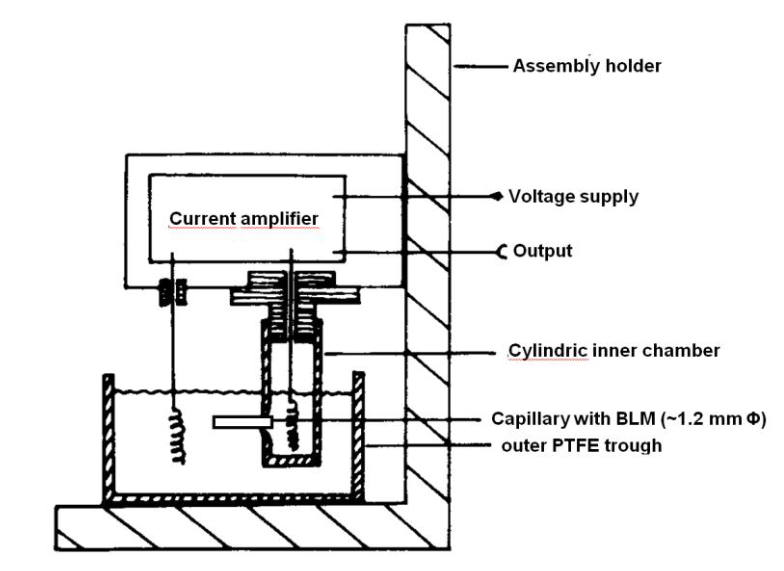
\includegraphics[width=.9\linewidth]{electrical setup.png}
  \caption{Electrical Setup}
  \label{fig:sub1}
\end{subfigure}%
\begin{subfigure}{.5\textwidth}
  \centering
  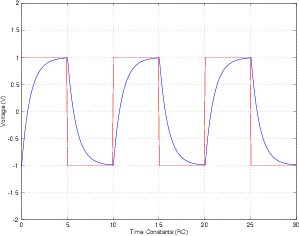
\includegraphics[width=.9\linewidth]{Square voltage + capacitor.png}
  \caption{Square AC + Capacitor}
  \label{fig:sub2}
\end{subfigure}
\caption{Electrical Observation}
\label{fig:test}
\end{figure}

Another manner for determining if a membrane was successfully built is trough visual inspection of the edge of the capillary trough a microscope. The optical set-up consists in focusing the microscope to the edge of the capillary and setting it at a certain angle relative to the perpendicular axis of the membrane, and then illuminating the same sample from a specular position relative to the perpendicular axis, this enables us to see the reflection of the light source on the sample trough the objective of the microscope.

If the optical setup is correctly tweaked and a membrane is formed at the tip of the capillary tube, then a characteristic optical phenomenon called \textit{Newton´s Rings} can be observed in the first minutes since the formation of the surface. After a few minutes the surface undergoes the Black Membrane phase and the effect presented in Figure 2.2 is no longer visible.

\begin{figure}[H]
    \centering
    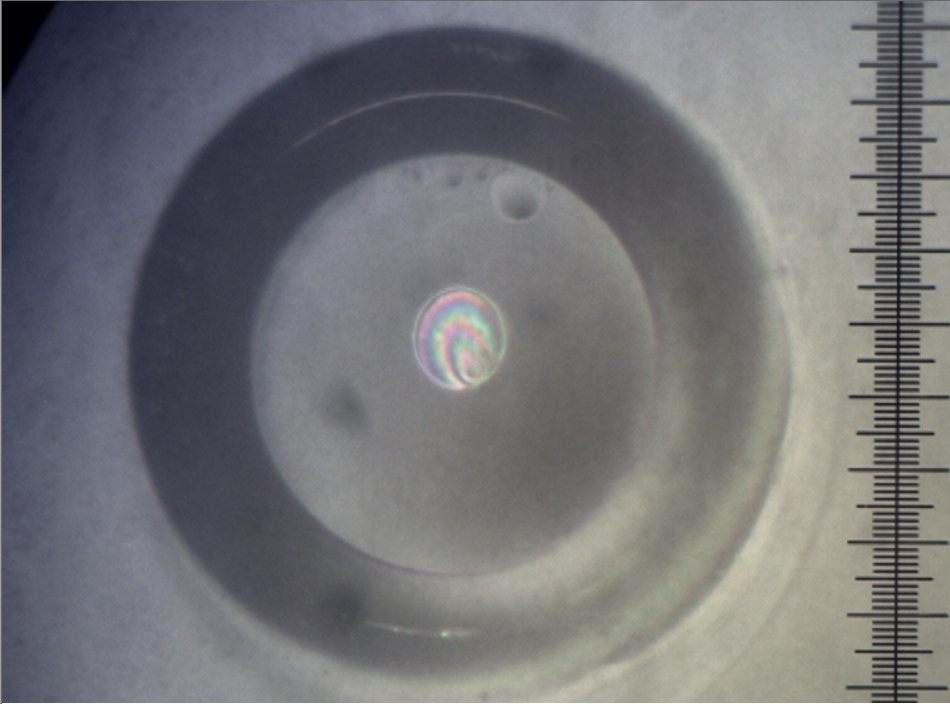
\includegraphics[width = 0.6\textwidth]{Group 8/Interference.PNG}
    \caption{Optical Observation}
    \label{fig:enter-label}
\end{figure}

\textbf{Determine the capacity, specific capacity and thickness of the membrane}
To determine the capacitance of this newly formed capacitor consisting of the black lipid membrane and the 2 water cells, we used the oscilloscope in combination with a known value resistor (100k$\Omega$ and a piece of software allowing us to extract $\tau$ ( RC time costant ) which is equal to the time required to discharge our capacitor to \( e^{-1} \)  trough the known resistor. In Figure 2.3 the green cursor is set to 36.8\% of the maximum current and we get the correpsonding value for tau of 0.0480 ms.

\begin{figure}[H]
    \centering
    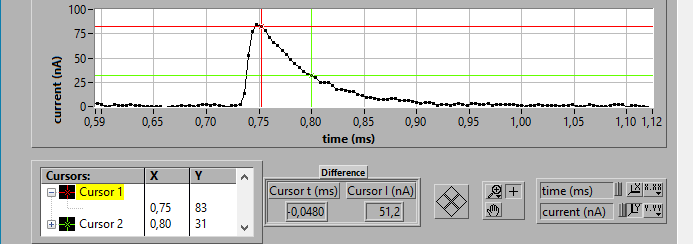
\includegraphics[width = 0.9\textwidth]{Group 8/Capacitance1.PNG}
    \caption{membrane Capacitance Software and $\tau$ at 10V, 250kHz sampling rate, 1000 samples}
    \label{fig:enter-label}
\end{figure}

Using formula 2.1, to solve for capacitance \( C \) with the values described above we get a final capacitance of 0.48 nF (nanoFarad)

\begin{equation}
C = \frac{\tau}{R}
\label{eq:capacitance}
\end{equation}

By using the formula for a parallel plate capacitor (see formula 2.2), which well fits with the bi-dimensionality of our lipid bilayer, the calculated capacitance of 0.48nF .
The Area was computed thanks to the scale in Figure 2.2, where each unit is 0.189 mm,  we measured the diameter to be 1.35 units ( from figure 2.2) which in turn gave us an area of 0.204mm² , the permittivity of vacuum $\varepsilon_0$ of 8.854 x 10-12 F/m and the assumed permittivity of lipid $\varepsilon$  of 2 F/m ( since a reference value for mono-olein is not published, even tough the chemical constituents are oleic acid and glycerol with 3 and 46.5 $\varepsilon$ respectively); we can therefore solve for d .


\begin{equation}
    C = \varepsilon * \varepsilon_0 \frac{A}{d} 
\label{eq:time_constant}
\end{equation}

In conclusion the thickness (d) of the membrane was established to be 7.52nm, the absolute error of this value was not computed but it should be noted that the order of magnitude corresponds with the one reported in other publications \cite{article} and we believe this is a notable feat considering that only macroscopic properties were recorded during the experiment.\\  

\textbf{Determine the membrane resistance and specific membrane conductivity}\\
%With the capacity of the membrane, we could apply equation Ohm´s law to acquire the resistance of the membrane, which is:
%\[
%R = \frac{V}{I} = 12.048 M\Omega
%\]
To determine the membrane resistance and specific membrane conductivity, we applied a  voltage of 50 mV across the membrane and measured the resulting current of the membrane to be 1.7 pA . The current-voltage (\textit{I-V}) relationship was recorded for the membrane.


From the \textit{I-V} relationship, the membrane resistance ($R_m$) was calculated using Ohm's Law:
\begin{equation}
R_m = \frac{V_m}{I_m} = 29.411 G\Omega
\end{equation}
where $V_m$ is the applied membrane voltage and $I_m$ is the measured current.


The specific membrane conductivity ($\sigma_m$) is the reciprocal of resistivity. To find $\sigma_m$, we used the membrane area ($A_m$)of 0.204mm² and thickness ($d_m$) of 7.52nm  :
\begin{equation}
\sigma_m = \frac{1}{R_m} \cdot \frac{d_m}{A_m} = 0.92 nS/m²
\end{equation}

\textbf{Determine the breakdown voltage and electric field in the membrane}

To determine the breakdown voltage (\(V_b\)), we should have incrementally increased the voltage applied across the membrane. We should have recorded the voltage at which a sudden, significant increase in current was observed, indicating membrane breakdown. This voltage is identified as the breakdown voltage.


The electric field (\(E\)) in the membrane is calculated using the measured breakdown voltage and the thickness of the membrane (\(d_m\)). The electric field is given by:
\begin{equation}
E = \frac{V_b}{d_m}
\end{equation}
where \(V_b\) is the breakdown voltage and \(d_m\) is the membrane thickness.

Our membrane broke down because of operation mistakes at a relatively low voltage ( 50mV)  which is far away from typical voltages expected from literature (300 mV) \cite{Benz1979}, this led us to the conclusion that our membrane broke because of other reasons instead of reaching the actual break down voltage. For this reason we cannot provide an Experimental result.

\subsection{Single channel measurements}
After observing the black lipid membrane and the exponential decay on the monitor, we changed the resistors from 100 k$\Omega$ and 500 k$\Omega$ to 100 M$\Omega$ and 500 M$\Omega$ to observe the pA scale of tiny current. The voltage was also changed to DC, 50mV for the following experiment. Then 5 \textmu l of gramidicin solution was suddenly injected around the membrane to form the ion channels. Then the software was used to record the current pattern. \\

\textbf{Modify the conductivity of the membrane by very low doping with gramicidin}

According to the equation 1.4, we could determine the conductivity under the single channle analysis (N$_p$(t) = 1):
\begin{equation}
    \Lambda = \frac{I_0}{V_M}
\end{equation}
Where I$_0$ is the current through the single channel. The current of the single channel is  1.7 pA (see next question), thus we could acquire the conductivtiy $\Lambda$ = $3.4 \times 10^{-11} \quad \Omega^{-1}$, which is close to the published value $3.0 \times 10^{-11} \quad \Omega^{-1}$. \cite{conductivity} \\

\textbf{Determine the single-channel current and analyze the distribution of channel
lifetimes}
%(histogram analysis)
The single channel current could be observed from the single-channel signals under low gramidicin concentration. Here the leakage current of the membrane should be considered, since it has a clearly influence to the measurement. In Figure 2.4, we could calculate that the single channel current is 3.4 pA (total current) - 1.7 pA (leakage current) = 1.7 pA (single channel current).
\begin{figure}[H]
    \centering
    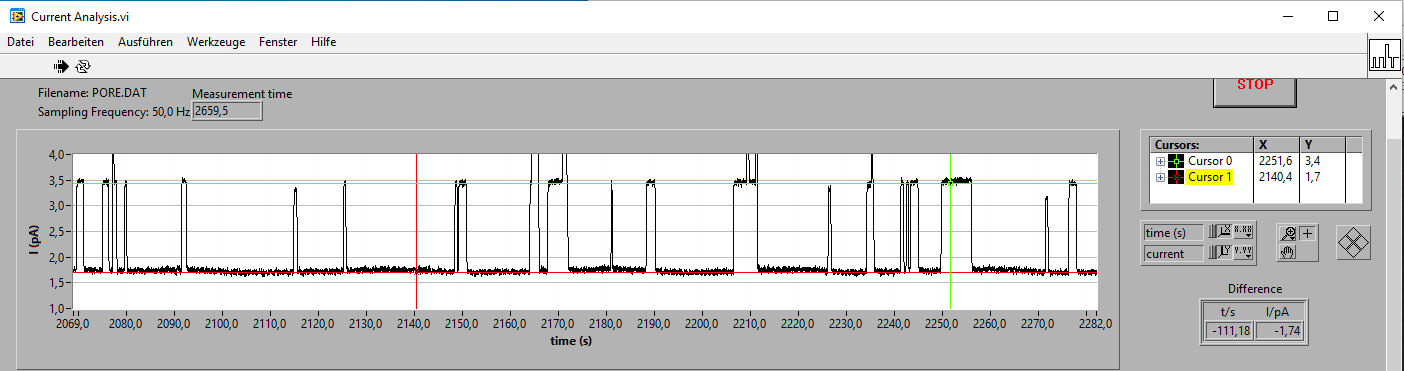
\includegraphics[width = 0.8\textwidth]{Group 8/Single Channel Current.PNG}
    \caption{The current-time plot of the single channel signals.}
    \label{fig:enter-label}
\end{figure}

Figure 2.5 tells the opening time distributions of the single channels. It follows the Poisson interval distribution. By fitting the curve, we could acquire the dissociation time of the gramidicin dimer($\tau$ = 2.15s, k$_D$ = 1/$\tau$ = 0.47s$^{-1}$), which is close to the published value ($\tau$ = 1.3s)\cite{dis_time}.
\begin{figure}[H]
    \centering
    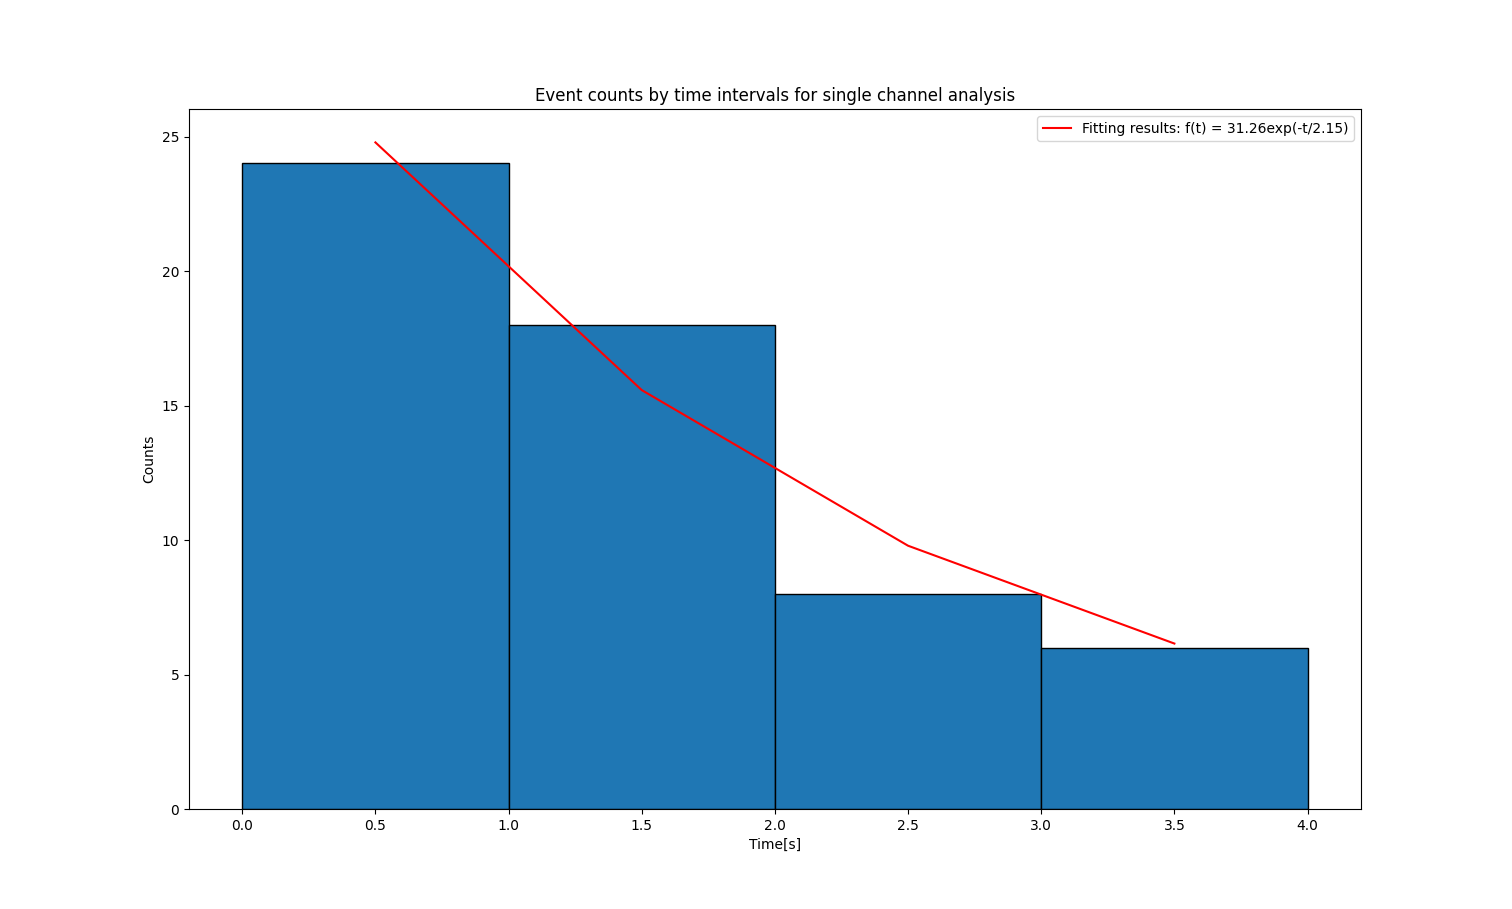
\includegraphics[width = 0.8\textwidth]{Group 8/poission.png}
    \caption{The opening time distributions and the exponential fitting of the single channels}
    \label{fig:enter-label}
\end{figure}

With this dissociation time, we could estimate how many ions were transferred through the channel during the lifetime of the channel:
\begin{equation}
    n = \frac{I \cdot \tau}{q} = 9.84\times 10^6 = 1.63 \times 10^{-17} mol
\end{equation}
Here the q is the charge of a single K$^+$ = 1.6 $\times$ 10$^{-19}$ C.\\

\textbf{Analyze the single-channel current at different membrane voltages. Is Ohm’s law
valid for single-channel currents?}\\
Unfortunately, in the experiment, we did not have time and chance to measure the single channel current at different membrane voltages. \\

\subsection{Measurements with multiple ion channels}


\textbf{Increase the gramicidin concentration in the membrane, so that several channels
are open at any time and multiple current steps are visible in the signal}\\
In the experiment, after a short time of the gramicidin injection, we observed that the current curve (Figure 2.6) changed from single steps to multi-steps, which indicated that more gramicidin was embedded in the membrane and formed dimer channels. 

\begin{figure}[H]
    \centering
    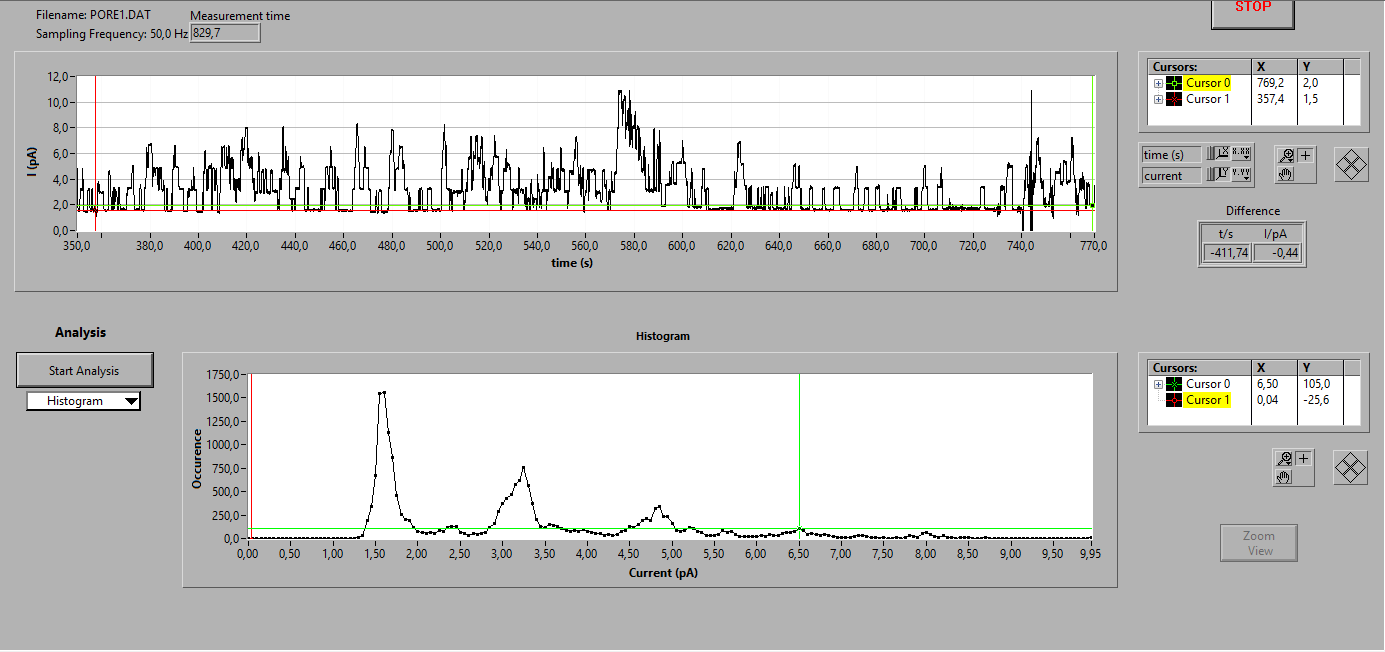
\includegraphics[width = 0.8\textwidth]{Group 8/Histogram2.PNG}
    \caption{The upper side is the  current-time plot under many channels open and close simultaneously. The lower side is the histogram of different currents.}
    \label{fig:enter-label}
\end{figure}
\textbf{Determine the single-channel current by analysis of the current histogram}\\

As is shown in the Figure 2.6, we could count the distribution of the different current levels. We could notice there are four major peaks, with current intensity 1.5 pA (leakage current), 3.3 pA (single channel current), 4.8 pA (double channel current) and 6.5 pA (triple channel current). With this, we could calculate the average single channel current $<i_0>$ = 1.67 pA.
\\

\subsection{Current fluctuation measurements}

\textbf{Increase the gramicidin concentration even more, so that many channel s are open
at any time and current steps in the signal are not visible any more}\\
Theoretically, we should further increase the concentration of the gramicidin and observe a curve as the Figure 2.7.

\begin{figure}[H]
    \centering
    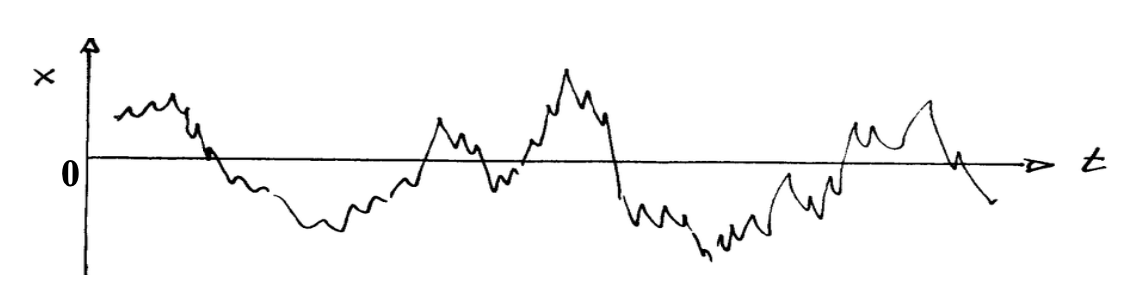
\includegraphics[width = 0.8\textwidth]{Group 8/theoritical plot of auto.png}
    \caption{The sketch of the typical curve shape for auto correlation analysis}
    \label{fig:enter-label}
\end{figure}

But after multiple additions of gramicidn, we couldn't achieve a concentration of channels in the membrane high enough to produce a plot similar to the one presented above in figure 2.7, this resulted in insufficient data for the autocorrelation analysis which greatly limited the results presente in Figure 2.8 .


\textbf{Determine the single-channel current and the average channel lifetime by
autocorrelation analysis of the fluctuating current}

During our experiment, the membrane broke before we could observe such a curve. As compensation, we applied the autocorrelation analysis on the curve so we could still distinguish multi-channels (Figure 2.8). 

\begin{figure}[H]
    \centering
    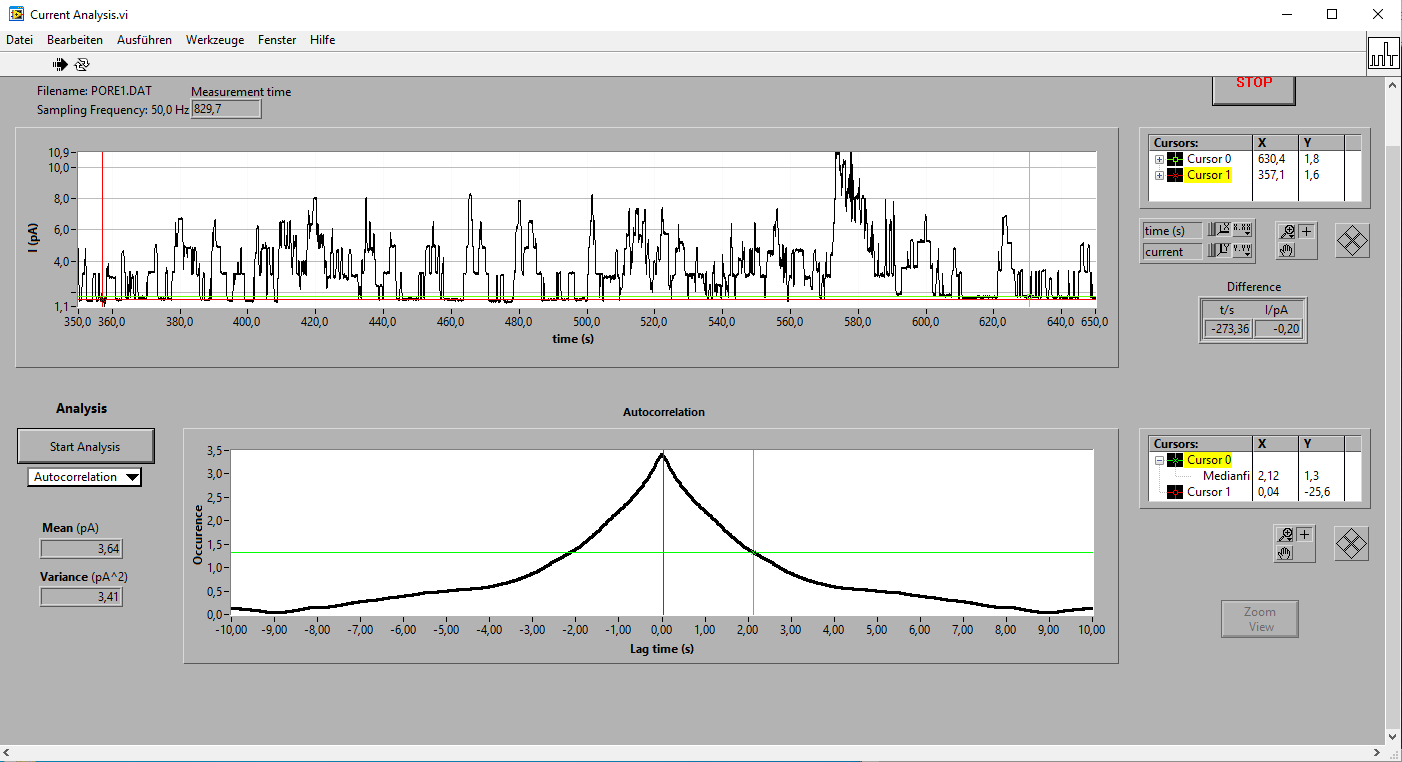
\includegraphics[width = 0.8\textwidth]{Group 8/Autocorrelation.PNG}
    \caption{Autocorrelation results of the current-time curve}
    \label{fig:enter-label}
\end{figure}

Using equation 1.7, we could acquire the relaxation time of the dimer $\tau$ = 2.08 s, and the dissociation time k$_D$ = 1/$\tau$ = 0.48/s. And we could also calculate the current of the single channel:
\[
<i_0> = \frac{\sigma^2_I}{<I_{ch}>} = \frac{\sigma^2_I}{<I> - I_{leak}} = \frac{3.41}{3.64-1.70}pA \approx 1.88pA
\]

\chapter{Discussion}
\label{cha:Discussion}
In this experiment, the single channel current was obtained using three different methods: 1.7 pA (single channel measurement), 1.67 pA (multiple channels measurement), and 1.88 pA (auto-correlation analysis). Overall, the results from all three methods are similar, indicating the accuracy of our measurements. Among these methods, the multiple channels measurement is the most precise because it can avoid experimental errors by directly observing and selecting the analysis interval, and it reduces errors through averaging the multichannel currents. The single channel measurement also provides a direct display of the current, whereas the auto-correlation analysis may produce a messy curve with unexpected signals that could influence the results. However, in our experiment, we still acquired a relatively good result with auto-correlation analysis. It is because that we used a non-typical current curve for auto-correlation, where the signals of different channels could still be distinguished and any obvious disturbances were already filtered out.\\

The dissociation time of the gramicidin dimers was obtained using the single channel measurement (2.15s) and auto-correlation analysis (2.08s). Both of them are close to the published data (1.3s). The differences between the published value and the measured values could be induced by insufficient data points. For single channel measurement, only four data points were used in the fitting. And for auto-correlation analysis, the density of the current signals were also lower than the typical one. However, comparing to the single channel measurement, the auto-correlation method used more data to acquire the dissociation time, thus it is also closer to the published value.

%The membrane broke for three times, so the measurement are on different membranes, that's one of the reason why they don't match with each other. 

%We don't have enough data for the auto correlation, which induce a larger error




\printbibliography

\chapter{Supplementary}
\label{cha:Supplementary}
\begin{figure}[H]
    \centering
    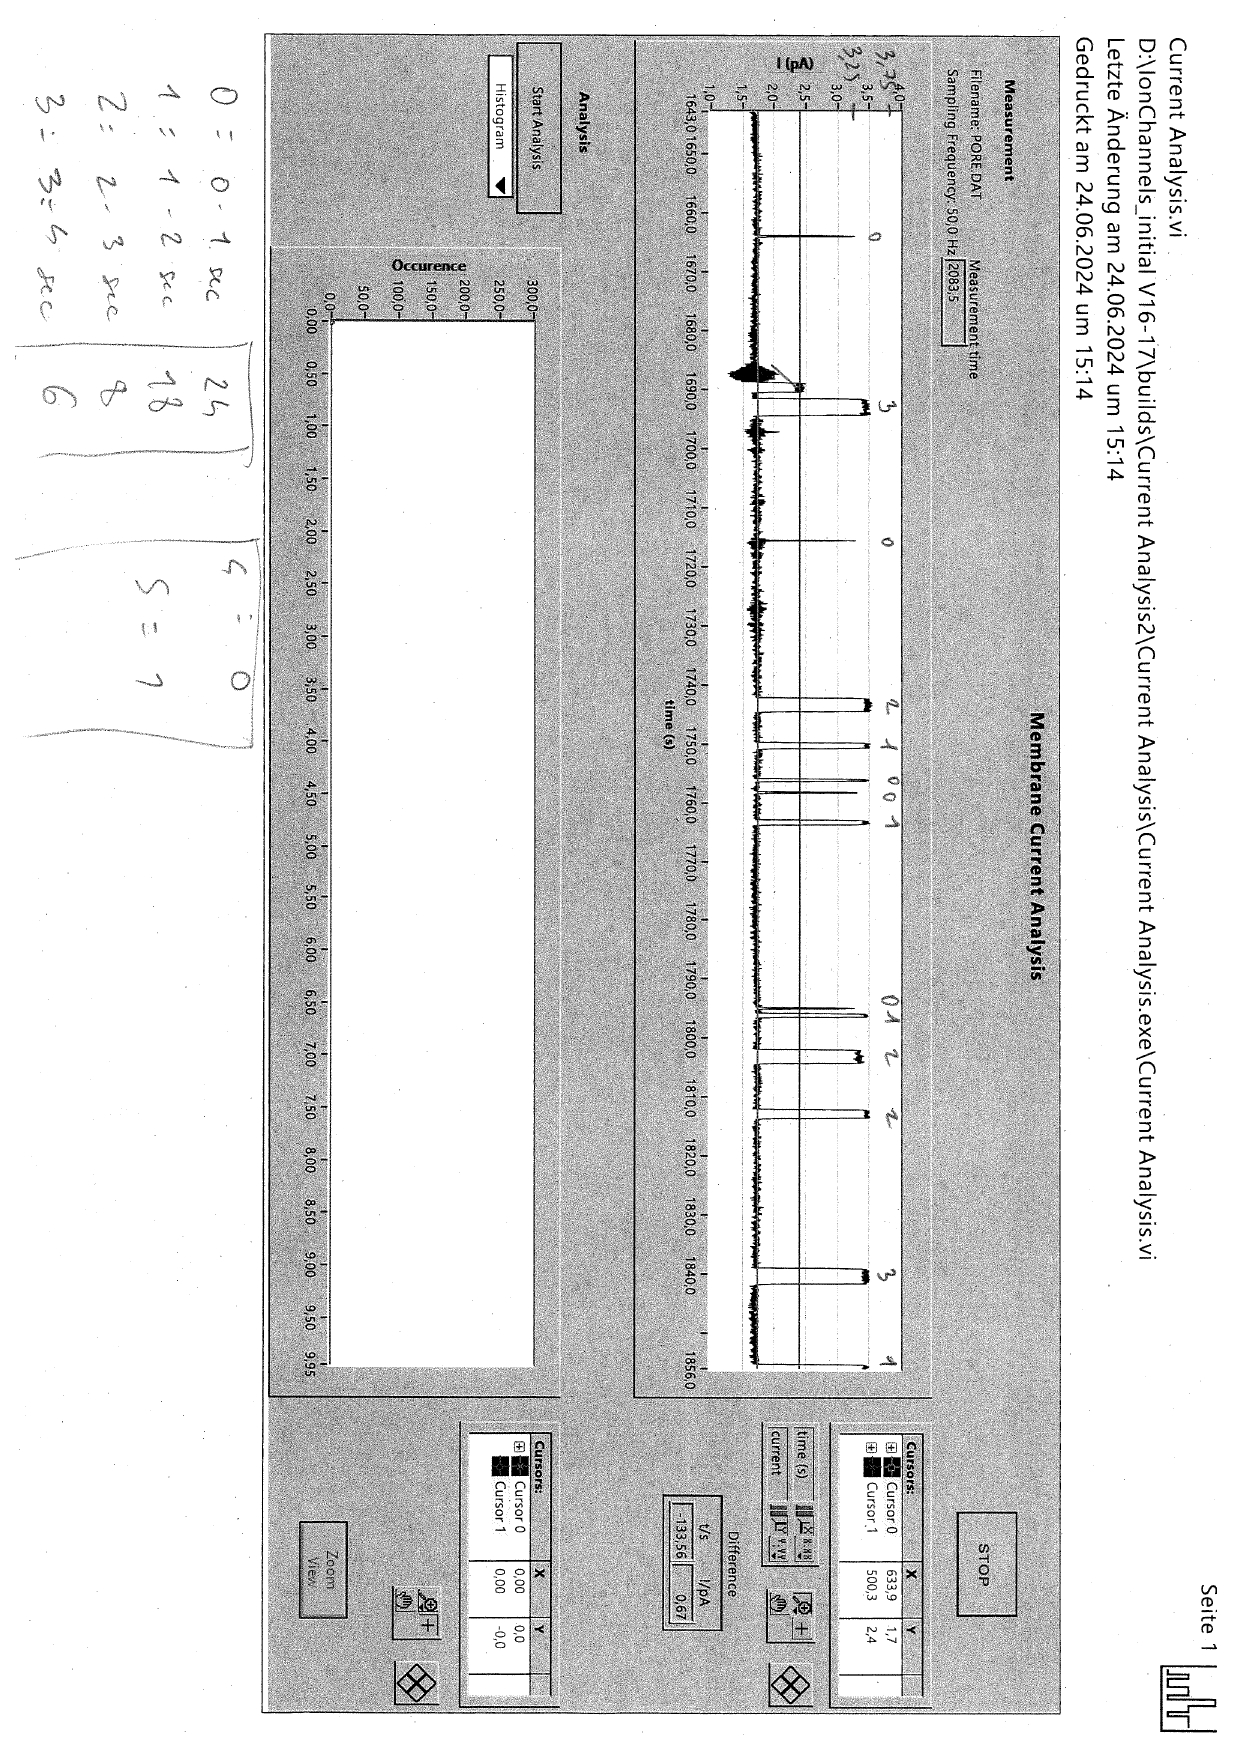
\includegraphics[angle=90,width = 0.9\textwidth]{Analysis/ilovepdf_pages-to-jpg/doc00131020240719122038-1_page-0001.jpg}
    \caption{Channels used for Statistics Fig 2.5}
    \label{fig:enter-label}
\end{figure}

\begin{figure}[H]
    \centering
    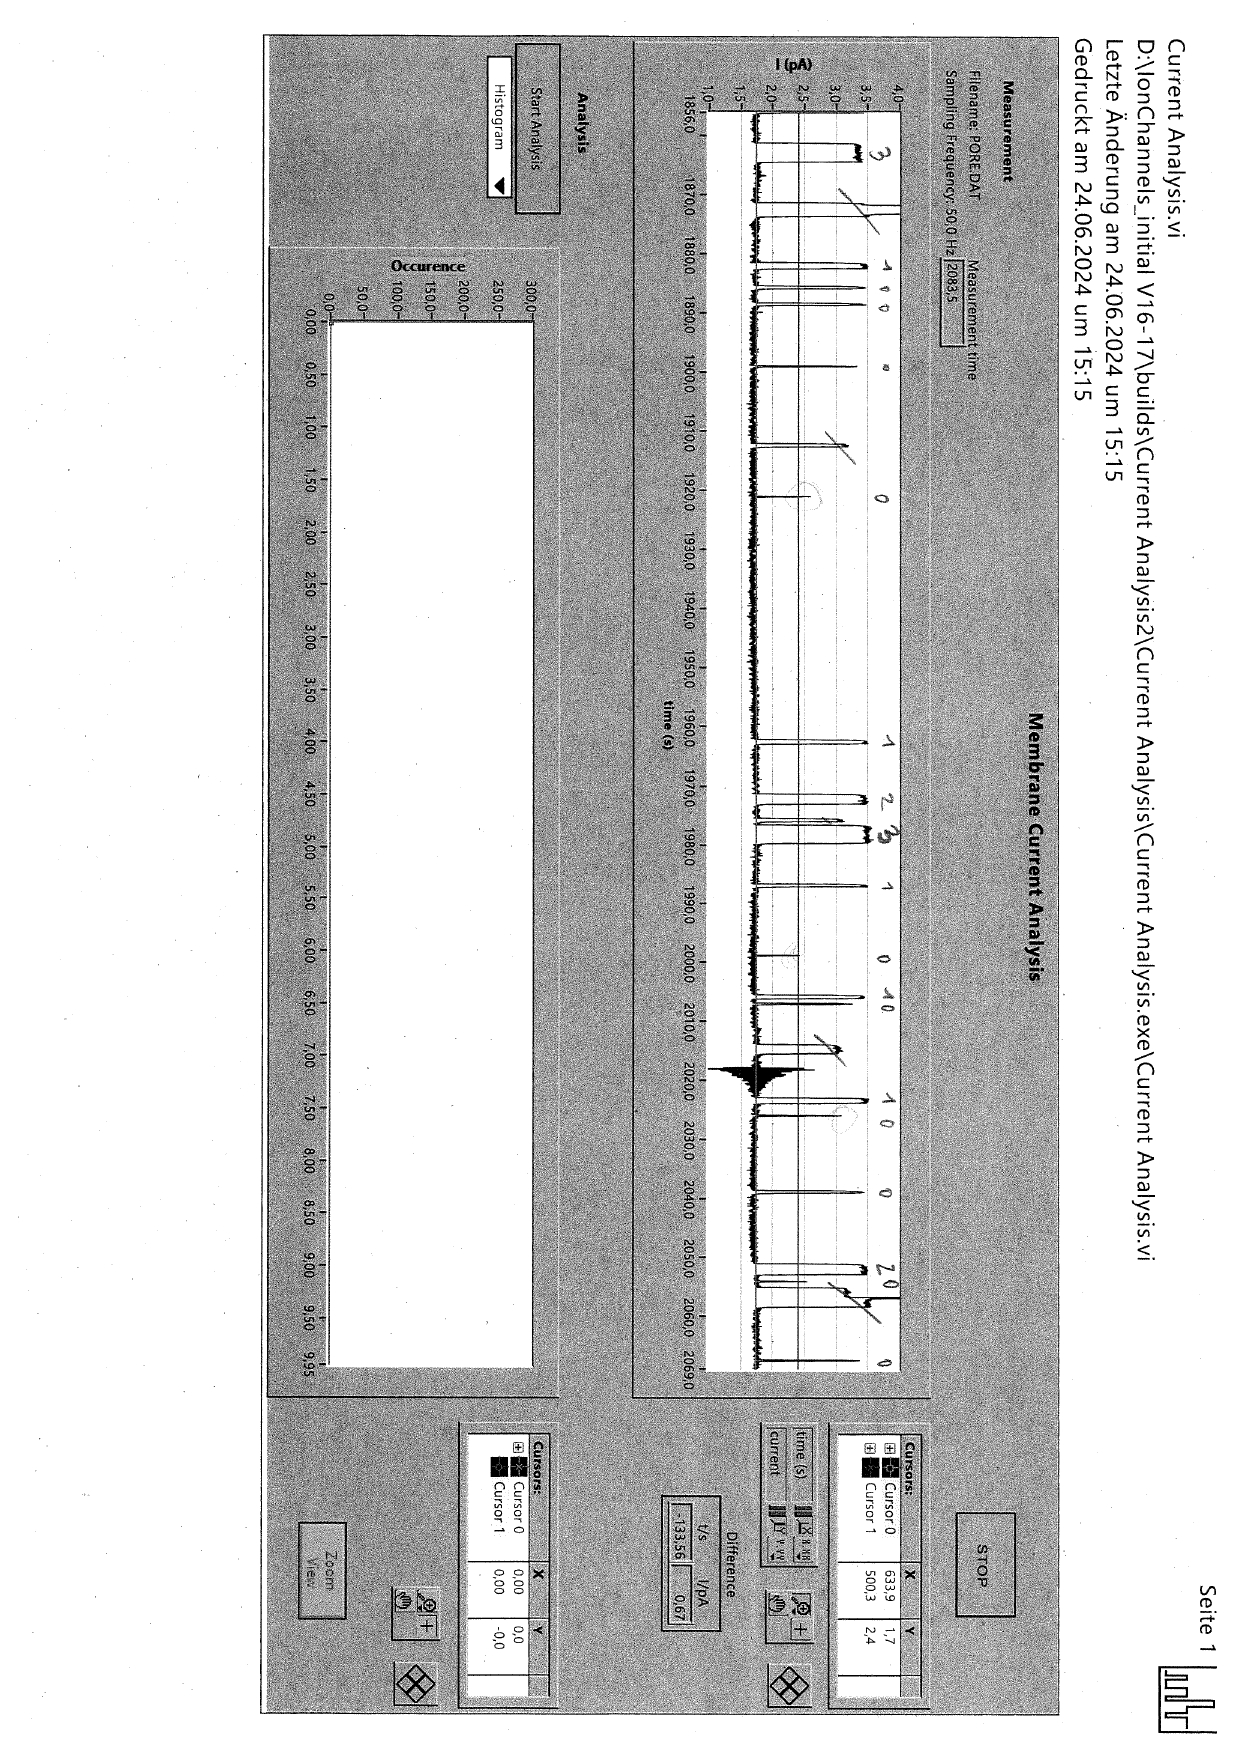
\includegraphics[angle=90,width = 0.9\textwidth]{Analysis/ilovepdf_pages-to-jpg/doc00131020240719122038-1_page-0002.jpg}
    \caption{Channels used for Statistics Fig 2.5}
    \label{fig:enter-label}
\end{figure}

\begin{figure}[H]
    \centering
    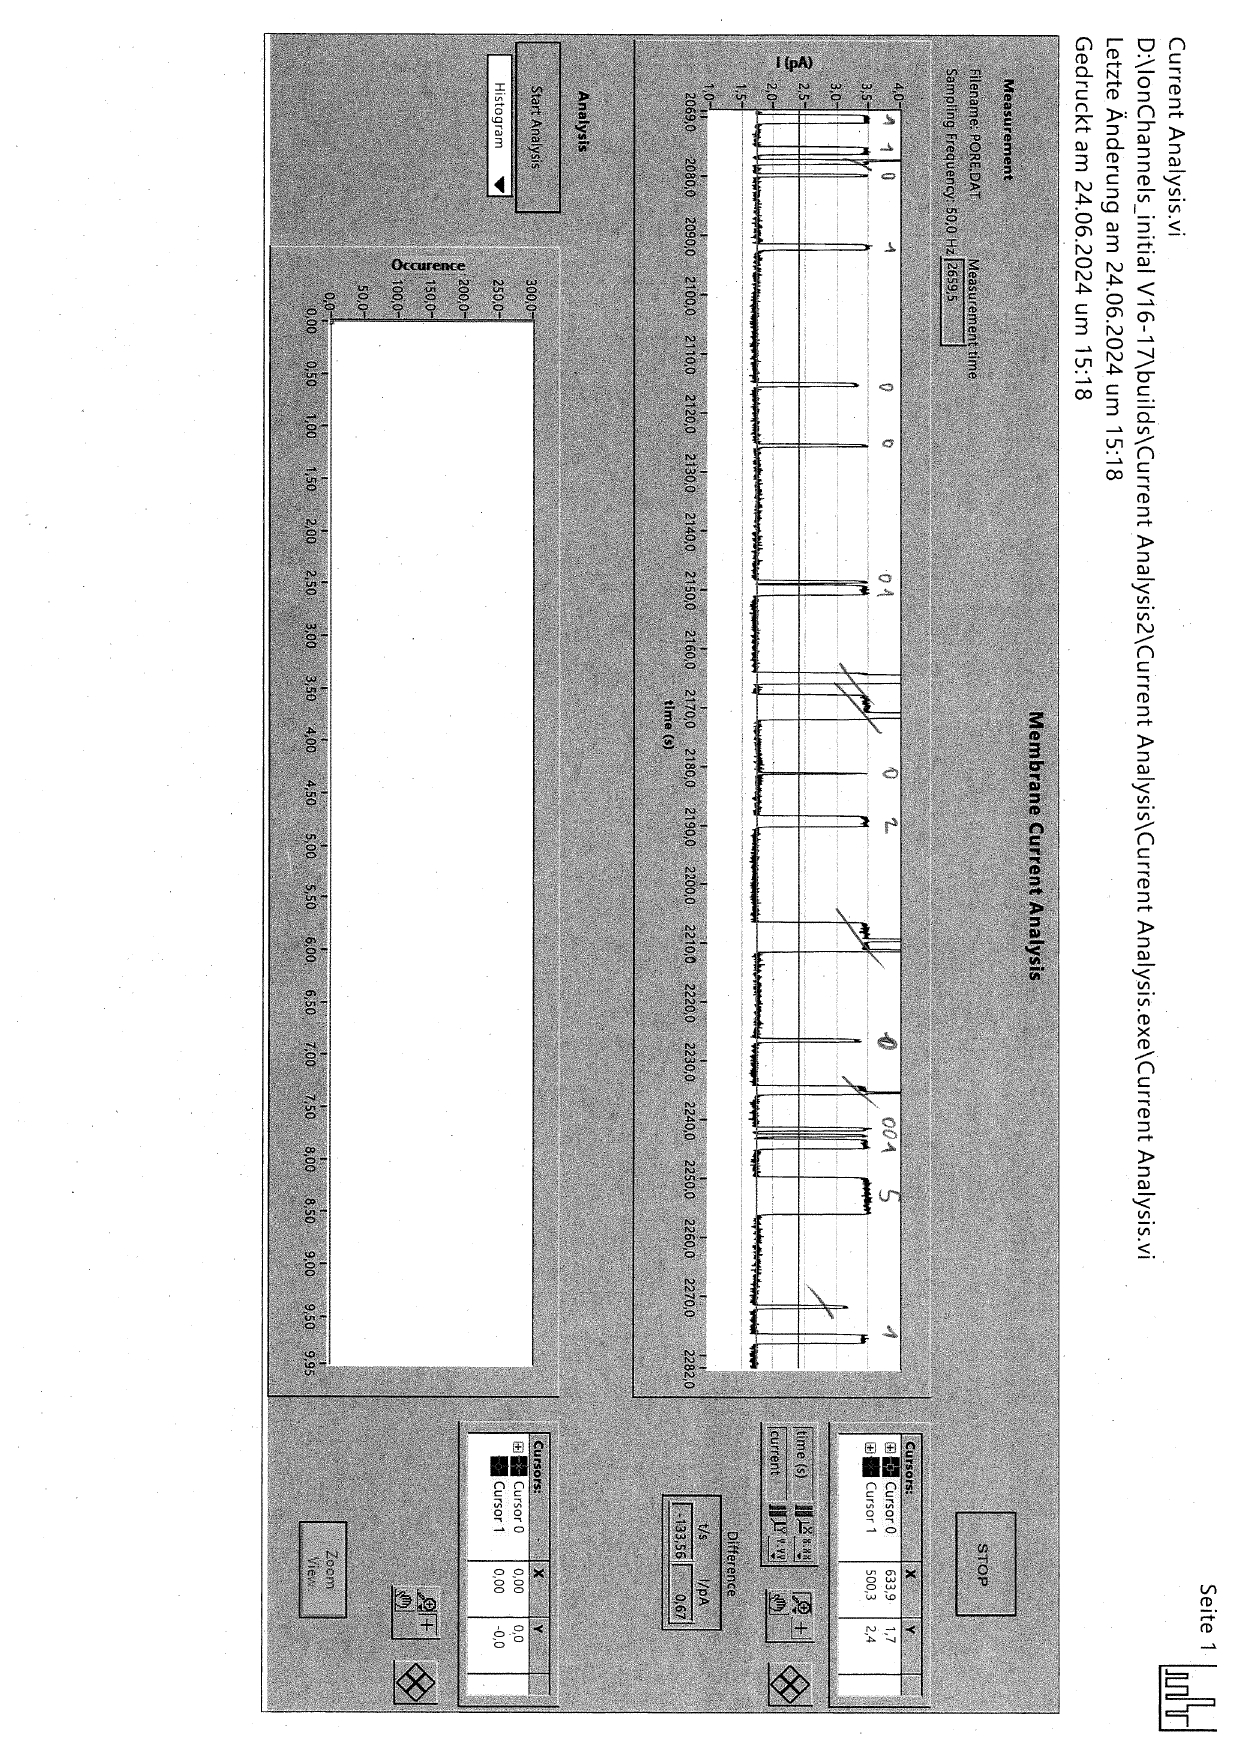
\includegraphics[angle=90,width = 0.9\textwidth]{Analysis/ilovepdf_pages-to-jpg/doc00131020240719122038-1_page-0003.jpg}
    \caption{Channels used for Statistics Fig 2.5}
    \label{fig:enter-label}
\end{figure}

\begin{figure}[H]
    \centering
    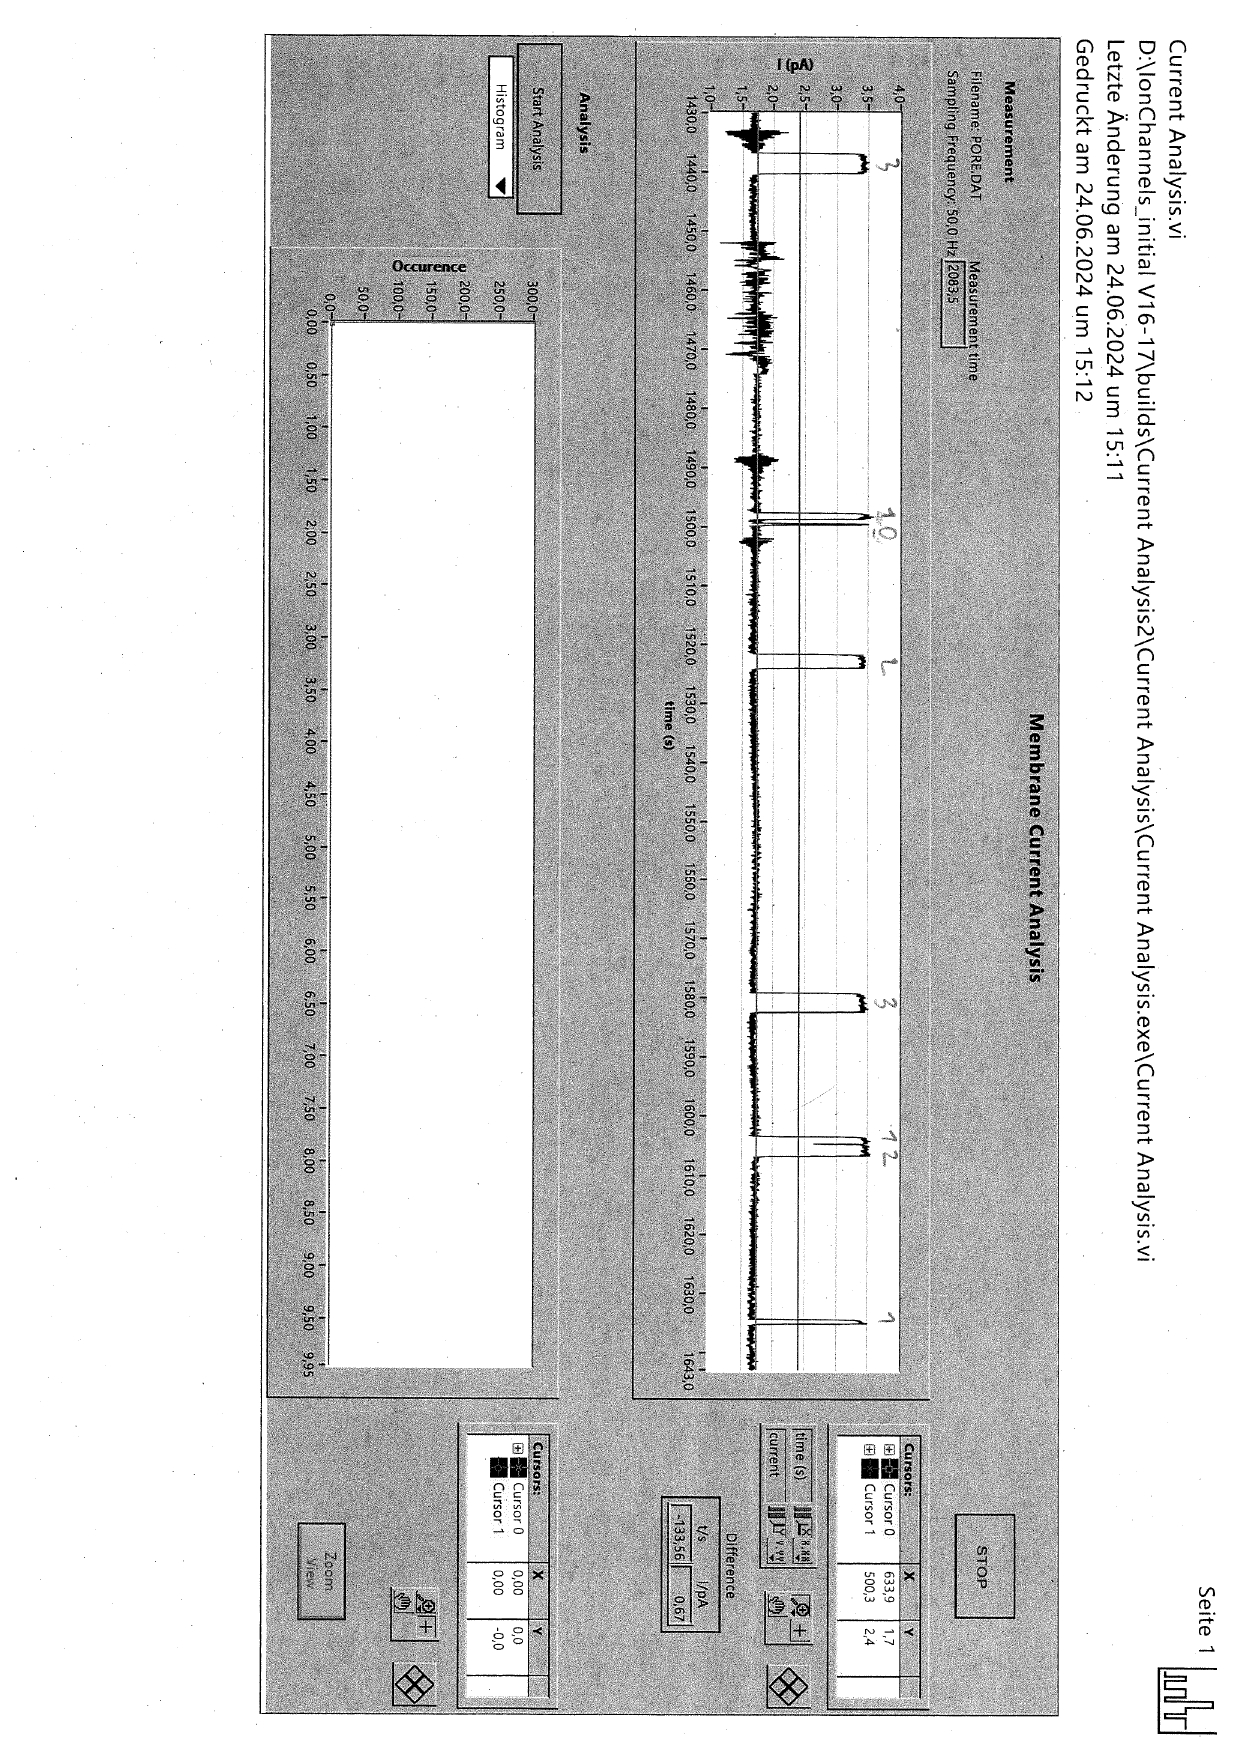
\includegraphics[angle=90,width = 0.9\textwidth]{Analysis/ilovepdf_pages-to-jpg/doc00131020240719122038-1_page-0004.jpg}
    \caption{Channels used for Statistics Fig 2.5 }
    \label{fig:enter-label}
\end{figure}
\end{document}
